\documentclass[tikz,border=7pt]{standalone}
\usepackage{amsmath}
\usetikzlibrary{arrows.meta,calc}
\definecolor{ink}{HTML}{21352F}
\definecolor{teal}{HTML}{087F7B}
\definecolor{gold}{HTML}{C58B2A}
\definecolor{blue}{HTML}{4B77A8}
\definecolor{rose}{HTML}{B65A62}
\definecolor{paper}{HTML}{FFFCF6}
\begin{document}
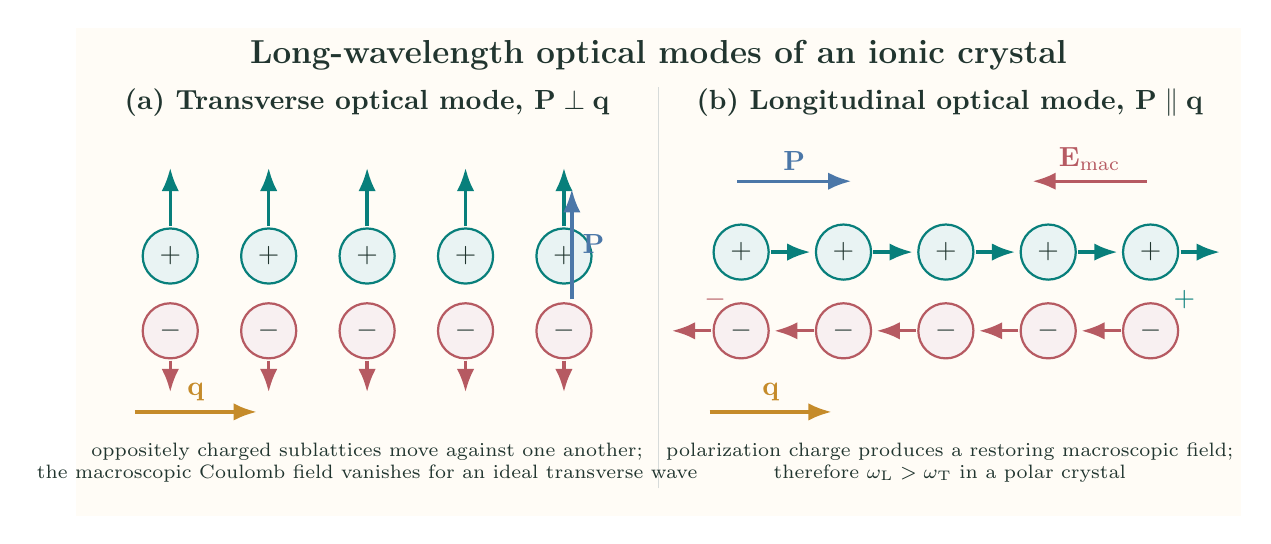
\begin{tikzpicture}[font=\sffamily,text=ink,>=Latex,
  ionp/.style={circle,draw=teal,thick,fill=teal!9,minimum size=7mm,inner sep=0pt},
  ionm/.style={circle,draw=rose,thick,fill=rose!9,minimum size=7mm,inner sep=0pt}]
  \fill[paper] (-7.4,-3.0) rectangle (7.4,3.2);
  \node[font=\bfseries\large] at (0,2.85) {Long-wavelength optical modes of an ionic crystal};
  \draw[ink!18] (0,-2.65)--(0,2.45);

  \node[font=\bfseries] at (-3.7,2.25) {(a) Transverse optical mode, $\mathbf P\perp\mathbf q$};
  \draw[->,very thick,gold] (-6.65,-1.68)--(-5.1,-1.68) node[midway,above] {$\mathbf q$};
  \foreach \x in {-6.2,-4.95,-3.7,-2.45,-1.2}{
    \node[ionp] at (\x,0.3) {$+$};
    \node[ionm] at (\x,-0.65) {$-$};
    \draw[->,teal,very thick] (\x,0.68)--(\x,1.42);
    \draw[->,rose,very thick] (\x,-1.03)--(\x,-1.43);
  }
  \draw[->,very thick,blue] (-1.1,-0.25)--(-1.1,1.15) node[midway,right] {$\mathbf P$};
  \node[font=\scriptsize,align=center] at (-3.7,-2.32) {oppositely charged sublattices move against one another;\\the macroscopic Coulomb field vanishes for an ideal transverse wave};

  \node[font=\bfseries] at (3.7,2.25) {(b) Longitudinal optical mode, $\mathbf P\parallel\mathbf q$};
  \draw[->,very thick,gold] (0.65,-1.68)--(2.2,-1.68) node[midway,above] {$\mathbf q$};
  \foreach \x in {1.05,2.35,3.65,4.95,6.25}{
    \node[ionp] at (\x,0.35) {$+$};
    \node[ionm] at (\x,-0.65) {$-$};
    \draw[->,teal,very thick] (\x+0.38,0.35)--(\x+0.88,0.35);
    \draw[->,rose,very thick] (\x-0.38,-0.65)--(\x-0.88,-0.65);
  }
  \draw[->,very thick,blue] (1.0,1.25)--(2.45,1.25) node[midway,above] {$\mathbf P$};
  \draw[->,very thick,rose] (6.2,1.25)--(4.75,1.25) node[midway,above] {$\mathbf E_{\rm mac}$};
  \node[rose,font=\bfseries] at (0.72,-0.25) {$-$};
  \node[teal,font=\bfseries] at (6.68,-0.25) {$+$};
  \node[font=\scriptsize,align=center] at (3.7,-2.32) {polarization charge produces a restoring macroscopic field;\\therefore $\omega_{\rm L}>\omega_{\rm T}$ in a polar crystal};
\end{tikzpicture}
\end{document}
